% Created 2024-07-08 Mon 22:16
% Intended LaTeX compiler: pdflatex
\documentclass[11pt]{article}
\usepackage[utf8]{inputenc}
\usepackage[T1]{fontenc}
\usepackage{ragged2e}
\usepackage{caladea}
\usepackage{graphicx}
\usepackage{longtable}
\usepackage{wrapfig}
\usepackage{rotating}
\usepackage{epigraph}
\usepackage[normalem]{ulem}
\usepackage{hyperref}
\usepackage{amsmath}
\usepackage{amssymb}
\usepackage{capt-of}
\usepackage{hyperref}
\usepackage{fancyhdr}
\title{Novena à Santa Bibiana}
 % \hypersetup{
 %  pdfauthor={},
 %  pdftitle={Novena a/à SANTO_NOME},
 %  pdfkeywords={},
 %  pdfsubject={},
 %  pdfcreator={Emacs 29.4 (Org mode 9.6.15)}, 
 %  pdflang={English}
 % }

\title{
  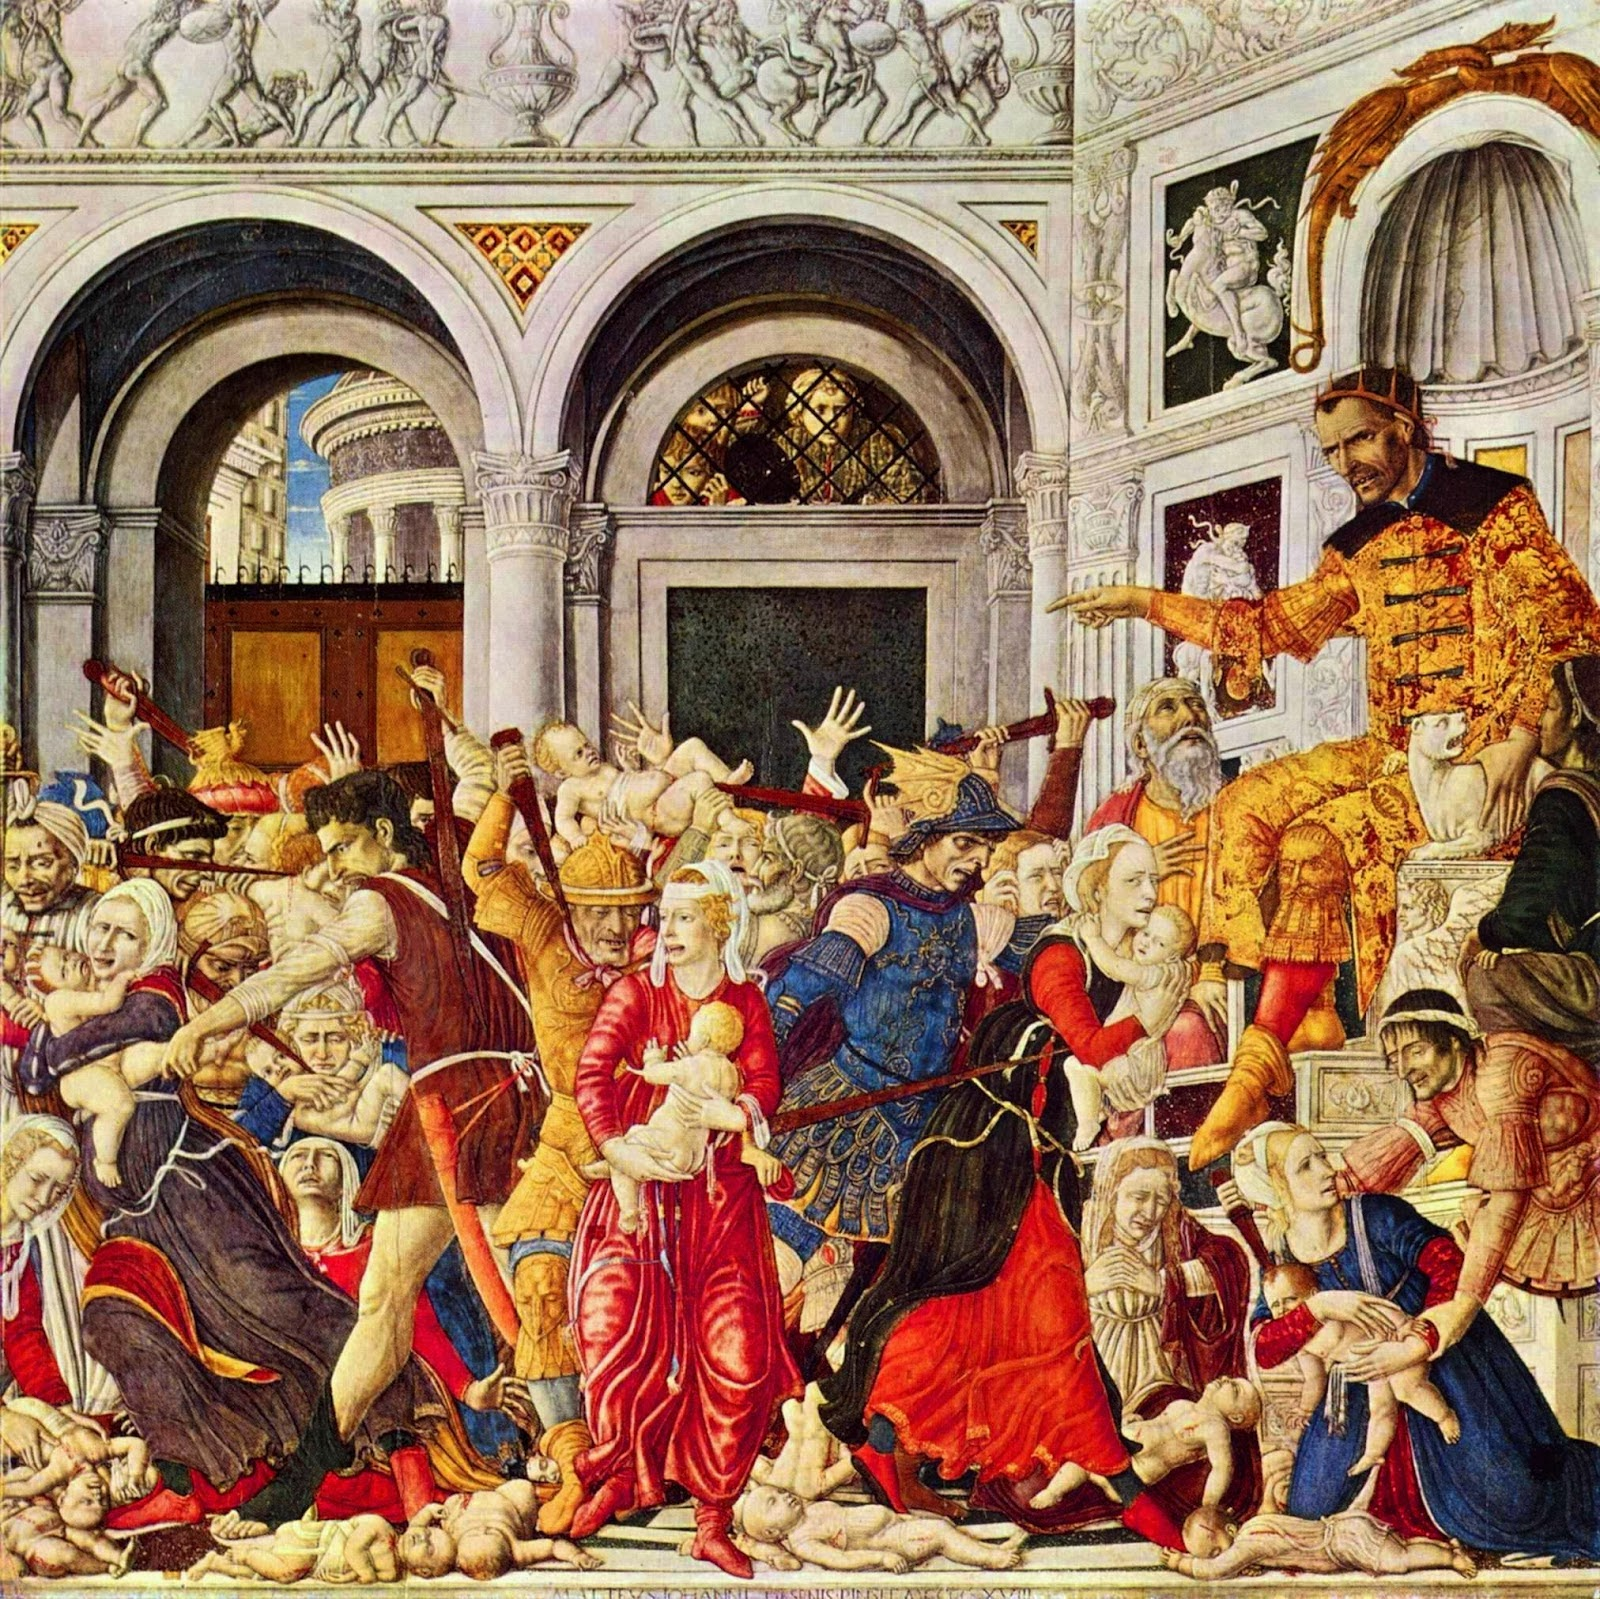
\includegraphics[scale=0.22]{./assets/imagem.jpg}
  \par
   NOVENA AOS SANTOS INOCENTES}
\author{Garamog, Nina Freitas}
\date{19/12 - 28/12}
\renewcommand{\contentsname}{Sumário}

\begin{document}
\maketitle

\thispagestyle{empty}

\pagestyle{fancy}
\fancyhf{} % clear existing header/footer entries
\fancyfoot[LO, CE]{
  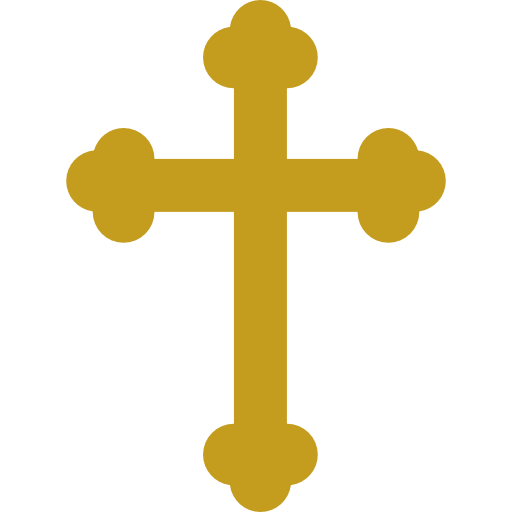
\includegraphics[scale=0.2]{./assets/cross.png}}

% Place Page X of Y on the right-hand
% side of the footer
\fancyfoot[R]{\thepage}
  
\newpage

\tableofcontents

\centering
\vfill
Visite-nos no Telegram: \url{https://t.me/CotidieNovena}
\newpage


\section{História}
\subsection*{\emph{Da boca dos pequeninos e das criancinhas de peito preparaste um louvor para ti” (Mt 21,16)}}\emph{}

\begin{justify}
No dia 28 de dezembro, a Igreja celebra os Santos Inocentes, ou seja, o martírio das crianças de Belém e arredores, massacradas por ordem de Herodes, que desejava matar o menino Jesus (Mt 2,16-18). Essa data é utilizada pelos grupos pró-vida para festejar a vida dos bebês e para protestar contra o aborto. A oração a seguir[1], distribuída em nove partes, pode ser recitada em forma de novena, ou ainda durante uma “marcha” ou procissão, com faixas e cartazes, como se costuma fazer em Anápolis, GO.
\end{justify}
\newpage

%%%%%%%%%%%%%%%%%%%%%%%%%%%%%%%%%%%%% Orações  %%%%%%%%%%%%%%%%%%%%%%%%%%%%%%%%%%%%%%%%%%%

\section{Orações}\label{sec:Orações} % (fold)

\subsection{Oração Inicial} % (fold)

“Meu Senhor, pelos Santos Inocentes, quero Vos rogar hoje por todos aqueles que são injustiçados, sofrem ameaças, são marginalizados e incompreendidos. Olhai pelos pequeninos, abandonados e assassinados pelas estruturas de morte de nossa sociedade. Que convosco eles alcancem dignidade e paz. Amém.”

\textbf{Pai Nosso, Avs Maria, Glória}

\subsection{Primeiro Dia}
\subsubsection*{I. O ódio de Herodes}

Herodes, chamado “o Grande”, vê-se incomodado pela notícia do nascimento do rei dos judeus, a quem os Magos procuravam para adorar e oferecer presentes. Como os Magos não voltaram a Jerusalém para lhe dizer quem era o Menino, Herodes decreta a morte de todos os meninos de até dois anos de idade, da cidade de Belém.

Ó Santos Inocentes, pequeninos, mortos por alguém que se julgava “grande”, intercedei a Deus em favor de tantos pequeninos, que continuamente são ameaçados pelo aborto, vítimas do ódio dos “grandes”. Amém.

\subsection{Segundo Dia}
\subsubsection*{II. Morrem por causa de Jesus}

Jesus veio para dar-nos a vida, mas ainda não era chegada a hora de sua Paixão e Morte. No lugar do Menino Jesus, que foge para o Egito com José e Maria, morrem as crianças de Belém. Derramam seu sangue por Cristo, que veio para derramar seu sangue por elas.

Ó Santos Inocentes, que derramastes vosso sangue por Cristo, antes mesmo que Cristo derramasse seu sangue por vós, intercedei a Deus para que não vacilemos diante das tribulações que sofremos por causa de Cristo, mesmo que elas cheguem até o martírio cruento. Amém.

\subsection{Terceiro Dia}
\subsubsection*{III. Ainda não falam, e já proclamam Cristo}

“Ninguém tem maior amor do que aquele que dá a vida por seus amigos” (Jo 15,13). Os Santos Inocentes ainda não sabem falar, mas dão testemunho de Cristo pela sua morte. Nós, que temos o dom da palavra, devemos falar de Cristo, viver como Cristo, mas sobretudo viver em Cristo e morrer com Cristo.

Ó Santos Inocentes, que proclamastes a glória de Deus não por palavras, mas pela própria morte, intercedei por nós a fim de que testemunhemos com a vida e com a morte aquilo que nossos lábios professam. Amém.

\subsection{Quarto Dia}
\subsubsection*{IV. Os sofrimentos dos pais}

As crianças de Belém morreram contra a vontade de seus pais, que deploraram a matança de seus filhos decretada por um rei tirano. As crianças vítimas do aborto nem sequer contam com o lamento de seus pais na hora da morte. Aqueles que mais deviam amá-las são os que procuram sua morte.

Ó Santos Inocentes, cuja morte causou tanta dor em vossos pais, intercedei a Deus por aqueles pais e mães que hoje, sem necessidade da ordem de um rei, voluntariamente procuram o aborto de seus filhos. Amém.

\subsection{Quinto Dia}
\subsubsection*{V. Os soldados executores}

Herodes não matou os bebês pessoalmente. Ordenou que soldados os matassem. Estes, embora vissem a monstruosidade da ordem do rei, preferiram obedecer-lhe, talvez por receio de receberem algum castigo. Hoje não são os governantes em pessoa quem pratica os abortos. Eles têm seus executores: toda uma equipe de profissionais espalhada em vários hospitais, sempre pronta a atender ao pedido das pessoas dispostas a abortar.

Ó Santos Inocentes, vítimas da covardia dos soldados executores da ordem de Herodes, intercedei a Deus por todos os médicos, enfermeiras e demais profissionais que, por medo de desagradar às autoridades, praticam aborto em nossos hospitais. Amém.

\subsection{Sexto Dia}
\subsubsection*{VI. O valor do sangue}

Nenhuma terra se envergonha de ter mártires. Roma não tem que se envergonhar por ter sido o local do martírio dos apóstolos Pedro e Paulo. A terra de Belém e seus arredores só têm que se gloriar de ter entre seus habitantes as crianças massacradas pela crueldade de um tirano. O sangue delas é sangue de bênção e de vida.

A situação muda totalmente quando se trata do sangue derramado em virtude de uma lei injusta, aprovada por parlamentares eleitos pelo povo. Quando uma nação, por meio de seus legisladores, ousa permitir a morte direta de inocentes, o sangue de tais vítimas, longe de atrair as bênçãos divinas, clama por castigo.

Ó Santos Inocentes, cujo sangue foi fonte de bênçãos para a cidade de Belém, intercedei a Deus para que nos livre da aprovação de uma lei permitindo o aborto em nosso país. Por vossa intercessão, livrai-nos do derramamento de um sangue de maldição e de morte em território brasileiro. Amém.

\subsection{Sétimo Dia}
\subsubsection*{VII. A inocência dos mártires}

Os mártires de Belém morreram sem terem cometido qualquer pecado. Morreram na inocência própria da infância. Hoje, as crianças que escapam do aborto, são ameaçadas com algo ainda pior: uma enxurrada de campanhas para corrompê-las e roubar-lhes a inocência. A televisão tornou-se veículo de pornografia. Nas escolas, o governo quer obrigá-las a aprender a usar preservativos. A indução dos pequeninos ao pecado supera a malícia do próprio aborto.

Ó Santos Inocentes, que derramastes vosso sangue conservando a inocência, intercedei a Deus em favor das criancinhas já nascidas, cuja inocência é ameaçada por uma avalanche de corrupção moral. Amém.

\subsection{Oitavo Dia}
\subsubsection*{VIII. As crianças que sobram}

Se Belém tivesse, ao tempo de Cristo, cerca de mil habitantes, talvez tenham morrido uns quarenta meninos. Na mente de Herodes, tais crianças não fariam falta. Poderiam morrer, contanto que, entre eles, estivesse o rei dos judeus, que ameaçava seu trono.

Hoje as clínicas de reprodução humana fabricam embriões humanos em grande quantidade. Os que não são implantados no útero, são congelados em nitrogênio líquido. São crianças que “sobram”. Não fazem falta. Por isso, o governo autoriza que sejam destruídas. E que seus restos mortais sejam usados para fins de “pesquisa”.

Ó Santos Inocentes, que morrestes após o nascimento, mas antes da idade adulta, intercedei a Deus para que não se fabriquem, não se manipulem nem se destruam os pequeninos em laboratório, em nome da medicina. Por vossa intercessão, que nenhuma criança seja considerada excedente ou descartável. Amém.

\subsection{Nono Dia}
\subsubsection*{IX. As crianças, imagem de Deus}

O desejo supremo do demônio é matar a Deus. Como Deus é imortal, ele investe contra a imagem de Deus, que é o homem. Por isso, o demônio é “homicida desde o princípio” (Jo 8,44). Entre os homens, os que mais e melhor refletem a imagem de Deus são as crianças. Isso explica o desejo insano de matá-las a qualquer custo. O que fez Herodes na época de Jesus, já havia feito o Faraó mais de mil anos antes. E hoje, o massacre se repete nas Casas Legislativas que deliberam sobre a morte dos inocentes.

Ó Santos Inocentes, cujo brilho nos olhos causou tanto ódio em quem odiava a Deus, intercedei por nós a fim de que não nos esqueçamos de que a luta contra o aborto é sobretudo uma luta espiritual contra o demônio, luta esta que requer o uso de armas espirituais. Amém.


\subsection*{Créditos:}
\href{https://www.nadateespante.com/products/novena-aos-santos-inocentes/}{Nada te Espante}


\end{document}
